\documentclass{beamer}
\usepackage{animate}
\usepackage{multimedia}
\usepackage[english,russian]{babel}

\usepackage{pgfpages}
\setbeameroption{show notes on second screen}
%https://tug.ctan.org/macros/latex/contrib/beamer/doc/beameruserguide.pdf

\usepackage{bm}


\usepackage[T2A]{fontenc}
\usepackage[utf8]{inputenc}

\setbeamertemplate{caption}[numbered]

\usetheme{CambridgeUS}
\usecolortheme{dolphin}

\title[Проектирование]{Проектирование}
\author[Быковских Д.А.]{Быковских Дмитрий Александрович}
\date{07.10.2023}

\begin{document}
	\begin{frame}
		\titlepage
	\end{frame}

	\begin{frame}{Преобразования и наблюдения}

		{\hfill
		Модельные координаты (МК)
		}
		
		Преобразование моделирования
		
		{\hfill
		Внешние координаты (ВК)
		}

		Преобразование наблюдения

		{\hfill
		Координаты наблюдения (КН)
		}

		Преобразование проектирования
		
		{\hfill
		Координаты проекции (КП)
		}
		
		Преобразование нормировки и отсечение
		
		{\hfill
		Нормированные координаты (НК)
		}

		Преобразование поля просмотра
		
		{\hfill
		Координаты устройства (КУ)
		}				
	\end{frame}

	\section{Математический взгляд}

	\begin{frame}{Общая информация}
		
		Проектирование --- преобразование, ставящее точки трехмерного пространства 
		в соответствие точки на плоскости. \\
		$f: R^3 \to R^2$
		
		Виды проектирования
		\begin{itemize}
			\item параллельные;
			\item перспективные.
		\end{itemize}

	\end{frame}

	\begin{frame}{Параллельное проектирование}
		\begin{columns}
			\begin{column}{0.5\textwidth}
			Плоскость проекции
			\[
				P: \bm{n} \cdot \bm{M} + d = 0	
			\]
			Лучи проектирования
			\[
				\bm{r} = \bm{r_0} + t \bm{l}	
			\]
			Должно выполняться условие
			\[
				\bm{n} \cdot \bm{l} \neq 0	
			\]
			Найдем точки пересечения
			\[
				\bm{n} \cdot (\bm{r_0} + t \bm{l}) + d = 0	
			\]
			\[
				t = -
				\frac{\bm{n} \cdot \bm{r_0} + d}{\bm{n} \cdot \bm{l}}
			\]
			\end{column}
			\begin{column}{0.5\textwidth}
				\begin{figure} 
						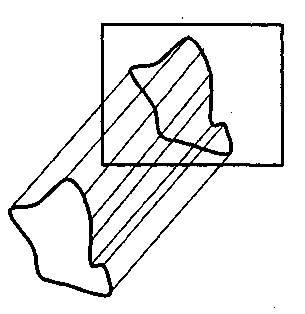
\includegraphics[width=0.8\textwidth]{images/parallel_projection.png}
					\caption{Схема параллельного проецирования}
				\end{figure}
			\end{column}
		\end{columns}
			
			\note{
					\begin{columns}
						\begin{column}{0.5\textwidth}
							\[
								P: \bm{n} \cdot (\bm{M} - \bm{M_0}) = 0	
							\]

							Откуда следует, что
							$
								d = - \bm{n} \cdot \bm{M_0}
							$
			\end{column}
			\begin{column}{0.5\textwidth}
				\begin{figure} 
					\href{https://function-x.ru/image/plane_pic01.jpg}{
						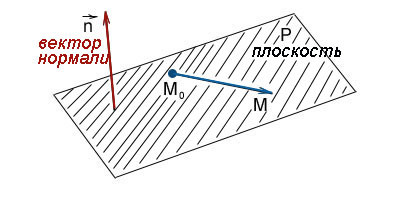
\includegraphics[width=0.6\textwidth]{images/plane.jpg}}
					\caption{Уравнение плоскости}
				\end{figure}
			\end{column}
		\end{columns}

			Векторное параметрическое уравнение прямой
			\[
				\bm{r}=\bm{r_0}+t\bm{l}	
			\]
			
			Параметрическое уравнение прямой
			\[
				\begin{cases} x=x_0+l_xt \\
					y=y_0+l_yt \\
					z=z_0+l_zt \\
					\end{cases}
			\]
			}

	\end{frame}

	\begin{frame}{Перспективное проектирование}

		\begin{columns}
			\begin{column}{0.5\textwidth}
			Плоскость проекции
			\[
				P: \bm{n} \cdot \bm{M} + d = 0	
			\]
			Лучи проектирования
			\[
				\bm{r} = (1-t) \bm{r_c} + t \bm{r_0}	
			\]
			Найдем точки пересечения
			\[
				\bm{n} \cdot [\bm{r_c} +t (\bm{r_0} - \bm{r_c}) ] + d = 0	
			\]
			\[
				t = -
				\frac{\bm{n} \cdot \bm{r_c} + d}{\bm{n} \cdot \bm{r_0} - \bm{n} \cdot \bm{r_c} }
			\]
			\end{column}
			\begin{column}{0.5\textwidth}
				\begin{figure} 
						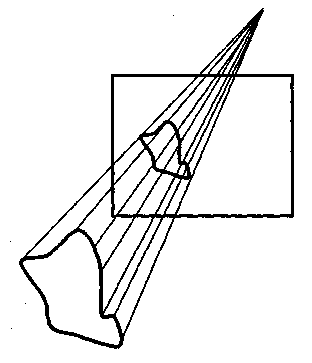
\includegraphics[width=0.8\textwidth]{images/perspective_projection.png}
					\caption{Схема перспективного проецирования}
				\end{figure}
			\end{column}
		\end{columns}
		\note{
			Проецирование называется перспективным, если проецирующие лучи, с помощью которых строится проекция предмета, исходят из одной точки.
		}
	\end{frame}

	\section{Проектирование}

	\begin{frame}{Проектирование}
		

		\begin{columns}
			\begin{column}{0.55\textwidth}

		Плоские геометрические проекции
		\begin{itemize}
			\item параллельные
			\begin{itemize}
				\item ортографические
				\begin{itemize}
					\item вид спереди
					\item вид сверху
					\item вид сбоку
				\end{itemize}
				\item аксонометрические
				\begin{itemize}
					\item триметрическая
					\item диметрическая
					\item изометрическая
				\end{itemize}
				\item косоугольные
				\begin{itemize}
					\item кавалье
					\item кабине 
				\end{itemize}
			\end{itemize}
			\item перспективные
			\begin{itemize}
				\item одноточечная
				\item двухточечная
				\item трехточечная
			\end{itemize}
		\end{itemize}

			\end{column}
			\begin{column}{0.45\textwidth}
				\begin{figure} 
						\includegraphics[width=\textwidth]{images/Comparison\_of\_graphical\_projections.png}
					\caption{Виды плоских проекций}
				\end{figure}
			\end{column}
		\end{columns}
		
		\note{

		В ортогональных (ортографических и акснометрических) проекциях направление проецирования является нормалью к проекционной плоскости (ортографическая и аксонометрическая);
		
		В косоугольных проекциях направление проецирования и нормаль к проекционной плоскости не совпадают.
		}
	\end{frame}

	\begin{frame}{Ортографические проекции}
	
		Самой простой из параллельных проекций, используемый обычно в инженерных чертежах. 

		Делится на 
		\begin{itemize}
			\item вид спереди (анфас);
			\item вид сверху (план);
			\item вид сбоку (профиль).
		\end{itemize}
		
		В этом случае точно изображаются правильные или «истинные» размер и форма одной плоской грани объекта.

		\[
			\begin{bmatrix}
				0 & 0 & 0 & 0 \\
				0 & 1 & 0 & 0 \\
				0 & 0 & 1 & 0 \\
				0 & 0 & 0 & 1 \\
			 \end{bmatrix}	
			 \qquad
		 \begin{bmatrix}
			1 & 0 & 0 & 0 \\
			0 & 0 & 0 & 0 \\
			0 & 0 & 1 & 0 \\
			0 & 0 & 0 & 1 \\
		 \end{bmatrix}
		 \qquad
		 \begin{bmatrix}
			 1 & 0 & 0 & 0 \\
			 0 & 1 & 0 & 0 \\
			 0 & 0 & 0 & 0 \\
			 0 & 0 & 0 & 1 \\
		 \end{bmatrix}
	 \]

		\note{
			\begin{figure} 
				\includegraphics[width=0.75\textwidth]{images/technical\_drawing.jpg}
			\caption{Пример чертежа}
		\end{figure}
		}
	
	\end{frame}

	\begin{frame}{Аксонометрические проекции}
		Строятся с помощью матриц поворота (углов Эйлера).
		\\ Виды
		\begin{itemize}
			\item Изометрическая проекция. \\
			В плоскости проекции углы между каждой парой осей равны.
			\item Диметрическая проекция. \\
			В плоскости проекции равны лишь 2 угла между осями.
			\item Триметрическая проекция. \\
			В плоскости проекции все 3 угла между собой различны.
		\end{itemize}
	\end{frame}
	
	\note{
		Аксонометрия в переводе с греческого обозначает измерение по осям.
		\[
			M_{r,y}(\phi) M_{r,x}(\theta) M_t =
		\]
		\[
			= 
		 \begin{bmatrix}
			 \cos \phi & 0 & - \sin \phi & 0 \\
			 0 & 1 & 0 & 0 \\
			 \sin \phi & 0 & \cos \phi & 0 \\
			 0 & 0 & 0 & 1 \\
		 \end{bmatrix}	
		 \begin{bmatrix}
			 1 & 0 & 0 & 0 \\
			 0 & \cos \theta  & \sin \theta & 0 \\
			 0 & -\sin \theta & \cos \theta & 0 \\
			 0 & 0 & 0 & 1 \\
		 \end{bmatrix}	
		 \begin{bmatrix}
			 1 & 0 & 0 & 0 \\
			 0 & 1 & 0 & 0 \\
			 0 & 0 & 0 & 0 \\
			 0 & 0 & 0 & 1 \\
		 \end{bmatrix}	
		 =
	 \]
	 \[
			= 
		 \begin{bmatrix}
			 \cos \phi & \sin \phi \sin \theta & 0 & 0 \\
			 0 & \cos \theta & 0 & 0 \\
			 \sin \phi & -\cos \phi \sin \theta & 0 & 0 \\
			 0 & 0 & 0 & 1 \\
		 \end{bmatrix}
	 \]

	}

	% \section{Преобразования наблюдения}
	\begin{frame}{Аксонометрическое проектирование}

		Коэффициенты искажения
		\[
			f_i = \sqrt{f_{i,x}^2+f_{i,y}^2+f_{i,z}^2}
		\]

		\[
		\begin{cases}
			f_x^2 = \cos^2 \phi + \sin^2 \phi \sin^2 \theta \\
			f_y^2 = \cos^2 \theta \\
			f_z^2 = \sin^2 \phi + \cos^2 \phi \sin^2 \theta \\
		\end{cases}	
		\]

		Для триметрической проекции
		\[
			f_x^2 \neq f_y^2 \neq f_z^2
		\]
		Для диметрической проекции
		\[
			f_x^2 = f_y^2 \neq f_z^2
		\]

		Для изометрической проекции
		\[
			f_x^2 = f_y^2 = f_z^2
		\]
		
		\note{
			коэффициенты сдвига
		}
		
	\end{frame}
	\begin{frame}{Аксонометрическое проектирование}

		\begin{columns}
			\begin{column}{0.45\textwidth}
		\[
			\begin{cases}
				f_x^2 = \cos^2 \phi + \sin^2 \phi \sin^2 \theta \\
				f_y^2 = \cos^2 \theta \\
				f_z^2 = \sin^2 \phi + \cos^2 \phi \sin^2 \theta \\
			\end{cases}	
		\]
		Изометрия
		\[
			f_x^2 = f_y^2 = f_z^2
			\qquad
			\begin{cases}
				f_x^2 = f_y^2  \\
				f_y^2 = f_z^2 \\
			\end{cases}	
		\]

		\[
			\sin^2 \phi  = \frac{\sin^2 \theta}{1 - \sin^2 \theta}
		\]


		\[
			\sin^2 \theta  = \frac{1}{3}
			\qquad
			\sin^2 \phi  = \frac{1}{2}
		\]

	\end{column}
	\begin{column}{0.55\textwidth}
		\begin{figure} 
				\includegraphics[width=\textwidth]{images/fallout\_2.jpg}
			\caption{Fallout}
		\end{figure}
	\end{column}
\end{columns}

		\note{
			{ \tiny
			\[
				\cos^2 \phi + \sin^2 \phi \sin^2 \theta = cos^2 \theta
			\]
			\[
				(1 - \sin^2 \phi) + \sin^2 \phi \sin^2 \theta = (1 - \sin^2 \theta)
			\]

			\[
				\sin^2 \theta - \sin^2 \phi + \sin^2 \phi \sin^2 \theta = 0
			\]

			\[
				\sin^2 \phi  = \frac{\sin^2 \theta}{1 - \sin^2 \theta}
			\]

			Теперь

			\[
				\sin^2 \phi +  \cos^2 \phi \sin^2 \theta = \cos^2 \theta 
			\]


			\[
				\sin^2 \phi + (1 - \sin^2 \phi) \sin^2 \theta = 1 - \sin^2 \theta
			\]

			\[
				\sin^2 \phi (1 - \sin^2 \theta)  = 1 - 2 \sin^2 \theta
			\]

			После подстановки

			\[
				\sin^2 \theta  = 1 - 2 \sin^2 \theta
			\]

			\[
				\sin^2 \theta  = \frac{1}{3}
			\]
		}
		}
	\end{frame}

	\begin{frame}{Косоугольное проектирование}
	\begin{columns}
		\begin{column}{0.45\textwidth}
			Проекция, где проектирующие прямые образуют с плоскостью проекции угол отличный от 90\textdegree.
			{ \scriptsize
			Поскольку проекционная плоскость перпендикулярна главной координатной оси, 
		то сторона объекта, параллельная этой плоскости, проецируется так, что можно измерить углы и расстояния. 
		При этом проецирование других сторон объекта также допускает проведение линейных измерений вдоль главных осей (но не угловых).
			}
		\end{column}
		\begin{column}{0.55\textwidth}
			\begin{figure} 
					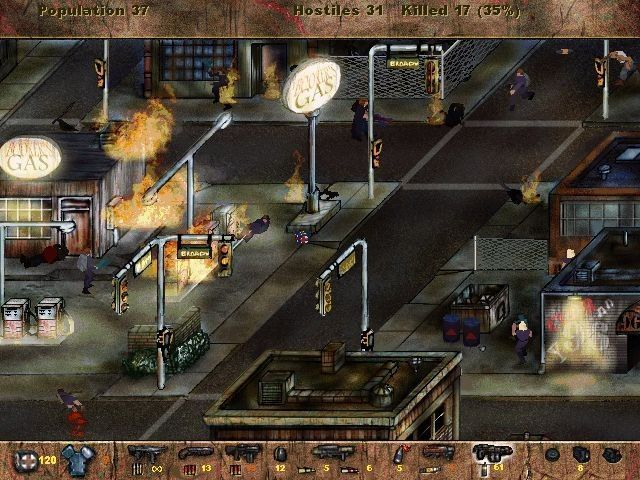
\includegraphics[width=\textwidth]{images/postal.jpg}
				\caption{Postal}
			\end{figure}
		\end{column}
	\end{columns}
	\note{
		\begin{figure} 
			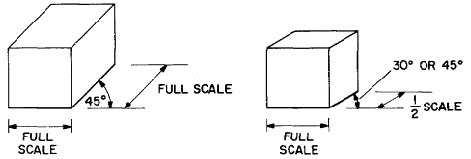
\includegraphics[width=\textwidth]{images/oblique.jpg}
		\caption{Косоугольные проекции: кавалье (слева); кабине (справа)}
	\end{figure}
	}
	\end{frame}

	\begin{frame}{Косоугольное проецирование}
		\begin{columns}
			\begin{column}{0.5\textwidth}
				\[
					\begin{bmatrix}
						1 & 0 & 0 & 0 \\
						0 & 1 & 0 & 0 \\
						-l \cos \alpha & - l \sin \alpha & 1 & 0 \\
						0 & 0 & 0 & 1 \\
					\end{bmatrix}	
				\]
			\end{column}
			\begin{column}{0.5\textwidth}
				\begin{figure} 
						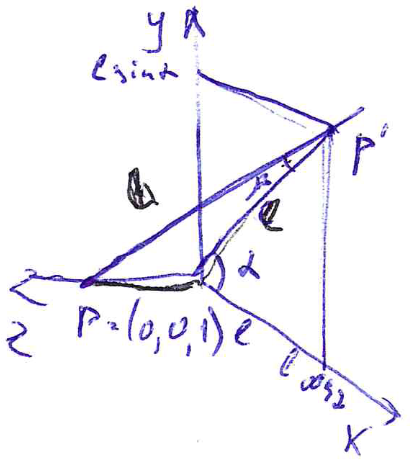
\includegraphics[width=0.7\textwidth]{images/oblique_sceme.png}
					\caption{Схема построения косоугольной проекции}
				\end{figure}
			\end{column}
		\end{columns}
		\note{

		}
	\end{frame}

	\begin{frame}{Перспективное проецирование}

		\begin{columns}
			\begin{column}{0.45\textwidth}
				Вид проекции, где лучи проектирования исходят из точки (центр проектирования), размещенной на конечном расстоянии от объектов и плоскости проектирования.
	
				\[
					\begin{bmatrix}
						1 & 0 & 0 & p \\
						0 & 1 & 0 & q \\
						0 & 0 & 1 & r \\
						0 & 0 & 0 & 1 \\
					\end{bmatrix}	
					,
				\]
					В этом случае точки фокуса имеют координаты:
					$c_x = (- \frac{1}{p},0,0)$,$c_y = (0,- \frac{1}{q},0)$, $c_z =(0,0, - \frac{1}{r})$
		\end{column}
		\begin{column}{0.55\textwidth}
			% https://studme.org/228266/informatika/osnovnye_svoystva_perspektivnoy_proektsii
			\begin{figure} 
					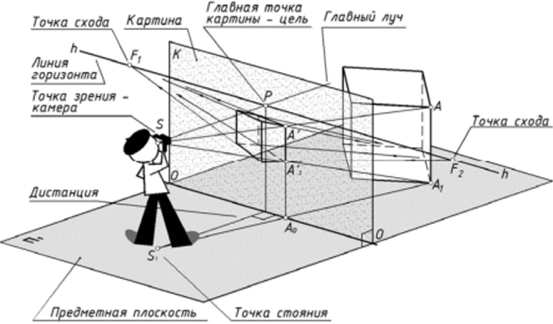
\includegraphics[width=\textwidth]{images/perspective_projections.png}
				\caption{Перспективная проекция}
			\end{figure}
		\end{column}
	\end{columns}

			\note{
				\[
					\begin{bmatrix}
						p_x^* \\
						p_y^*	\\
						p_z^* \\
						1			\\
					\end{bmatrix}^T
					\neq
					\begin{bmatrix}
						p_x \\
						p_y	\\
						p_z \\
						1		\\
					\end{bmatrix}^T	
					\begin{bmatrix}
						1 & 0 & 0 & 0 \\
						0 & 1 & 0 & 0 \\
						0 & 0 & 1 & r \\
						0 & 0 & 0 & 1 \\
					\end{bmatrix}
					\begin{bmatrix}
						1 & 0 & 0 & 0 \\
						0 & 1 & 0 & 0 \\
						0 & 0 & 0 & 0 \\
						0 & 0 & 0 & 1 \\
					\end{bmatrix}
					=
					\begin{bmatrix}
						p_x \\
						p_y	\\
						0 \\
						p_z \cdot r+1		\\
					\end{bmatrix}^T
				\]
				
				\[
					\begin{bmatrix}
						\frac{p_x}{p_z \cdot r+1} \\
						\frac{p_y}{p_z \cdot r+1} \\
						0 \\
						1	\\
					\end{bmatrix}^T
					=					
					\begin{bmatrix}
						p_x^* \\
						p_y^*	\\
						p_z^* \\
						1			\\
					\end{bmatrix}^T
				\]
		
				\[
					\begin{bmatrix}
						1 & 0 & 0 & p \\
						0 & 1 & 0 & q \\
						0 & 0 & 1 & r \\
						0 & 0 & 0 & 1 \\
					\end{bmatrix}	
					\qquad
					\to
					\qquad
					\begin{bmatrix}
						\frac{p_x}{p_x \cdot p + p_y \cdot q + p_z \cdot r+1} \\
						\frac{p_y}{p_x \cdot p + p_y \cdot q + p_z \cdot r+1} \\
						0 \\
						1	\\
					\end{bmatrix}^T
					=					
					\begin{bmatrix}
						p_x^* \\
						p_y^*	\\
						p_z^* \\
						1			\\
					\end{bmatrix}^T
				\]

			}
	\end{frame}
	\begin{frame}{Перспективное проецирование}

		\begin{figure} 
			% 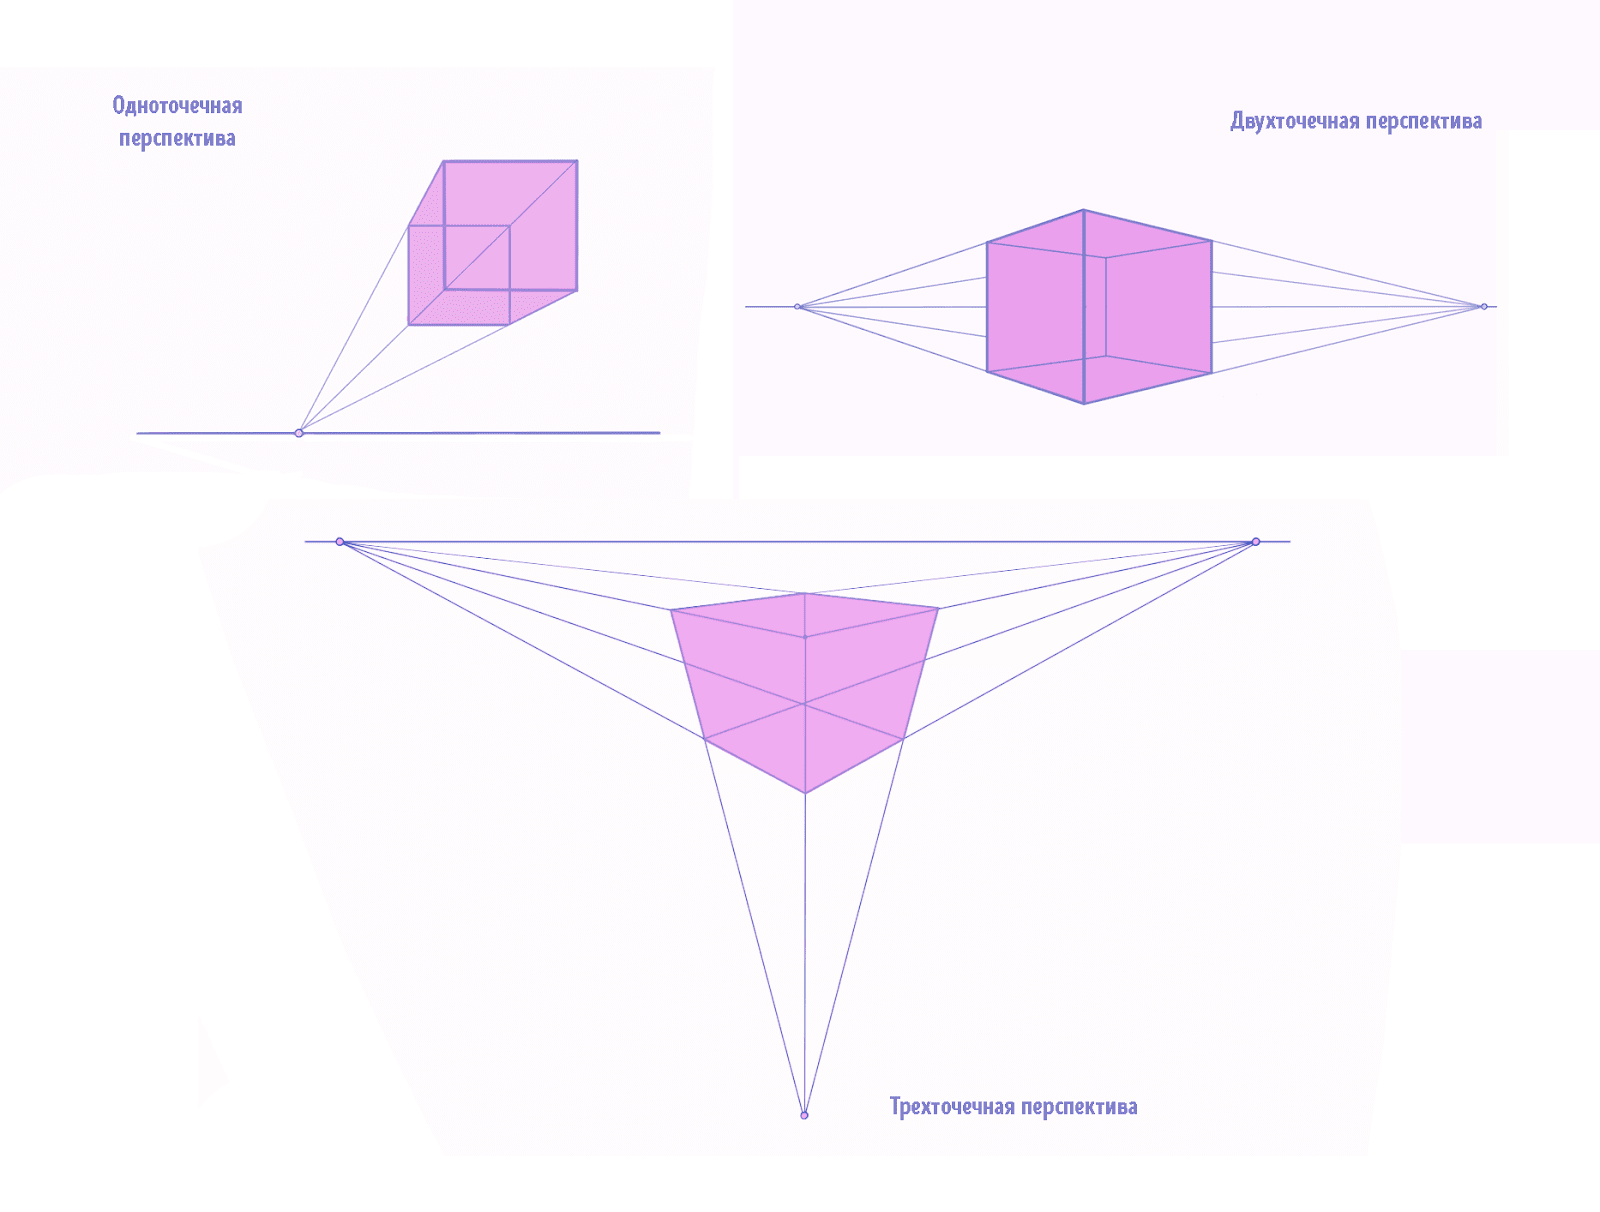
\includegraphics[width=0.65\textwidth]{images/1-2-3-point.png}
			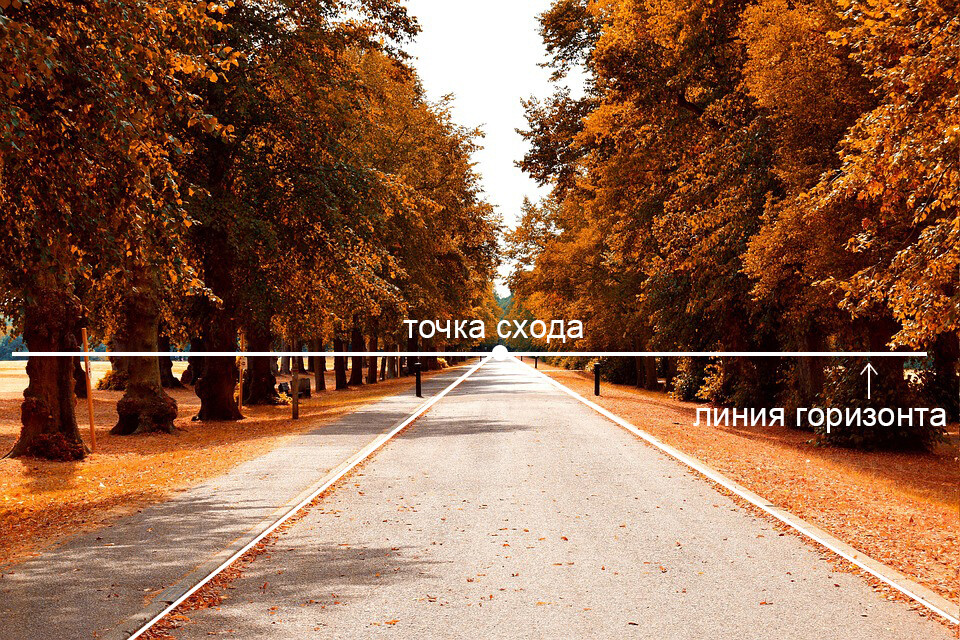
\includegraphics[width=0.33\textwidth]{images/1-point.jpeg}
			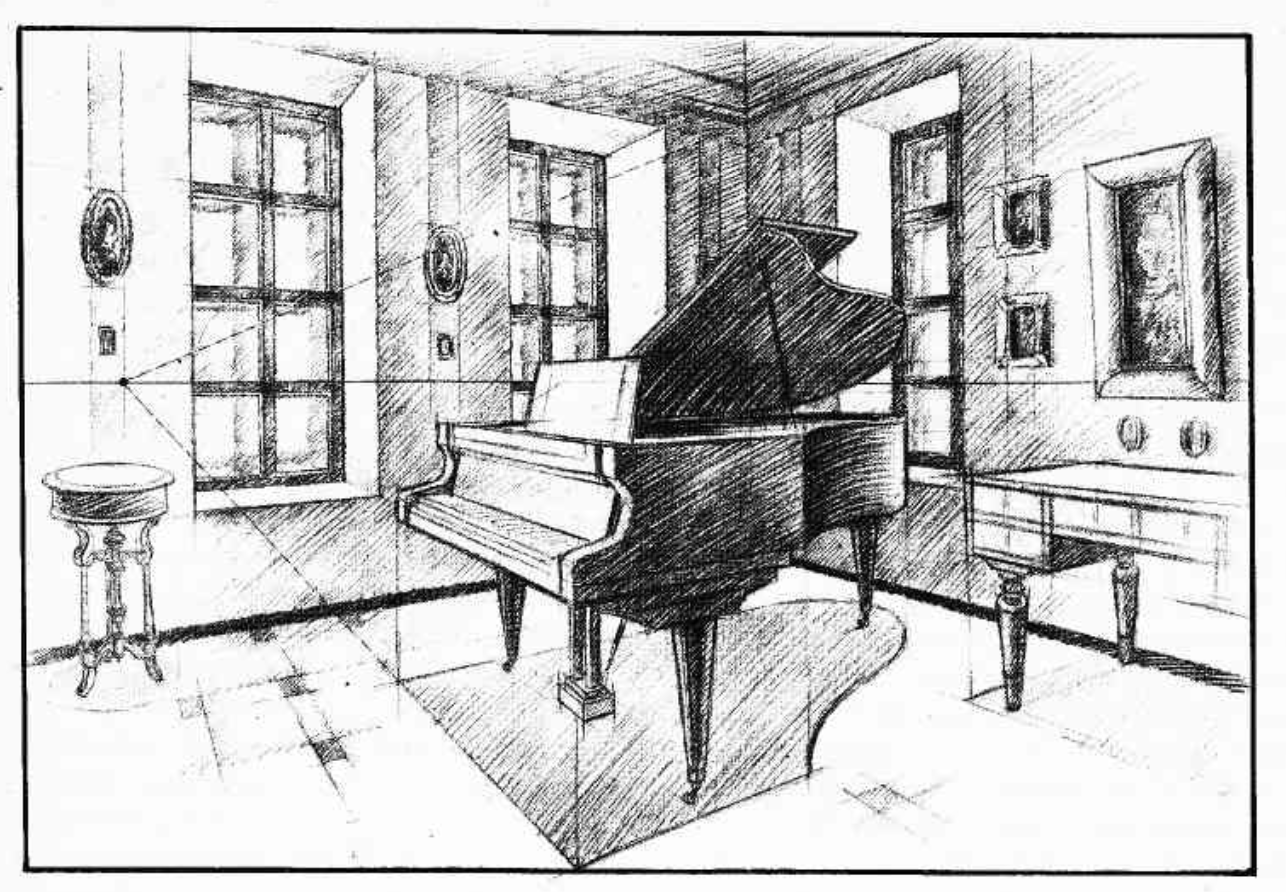
\includegraphics[width=0.33\textwidth]{images/2-point.png}
			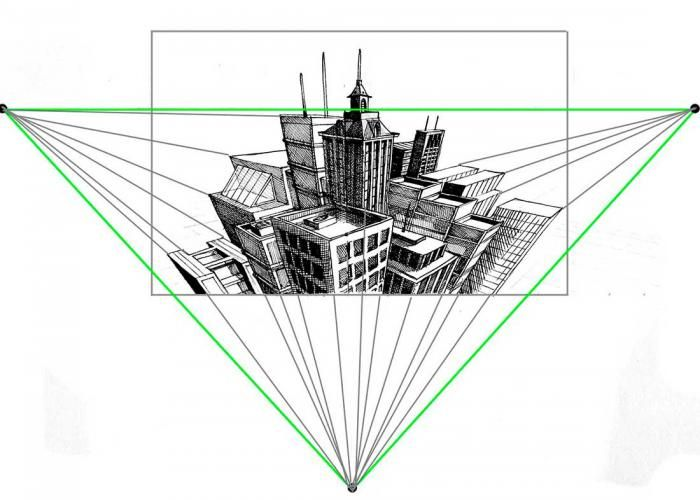
\includegraphics[width=0.4\textwidth]{images/3-point.jpg}
			\caption{Виды перспективных проекций: одноточечная (фронтальная), двухточечная (угловая), трехточечная (вертикальная)}
		\end{figure}

		\note{
			\begin{figure} 
				\href{https://smirnov.school/blog/gameart/chto-takoe-linejnaya-perspektiva/}{
				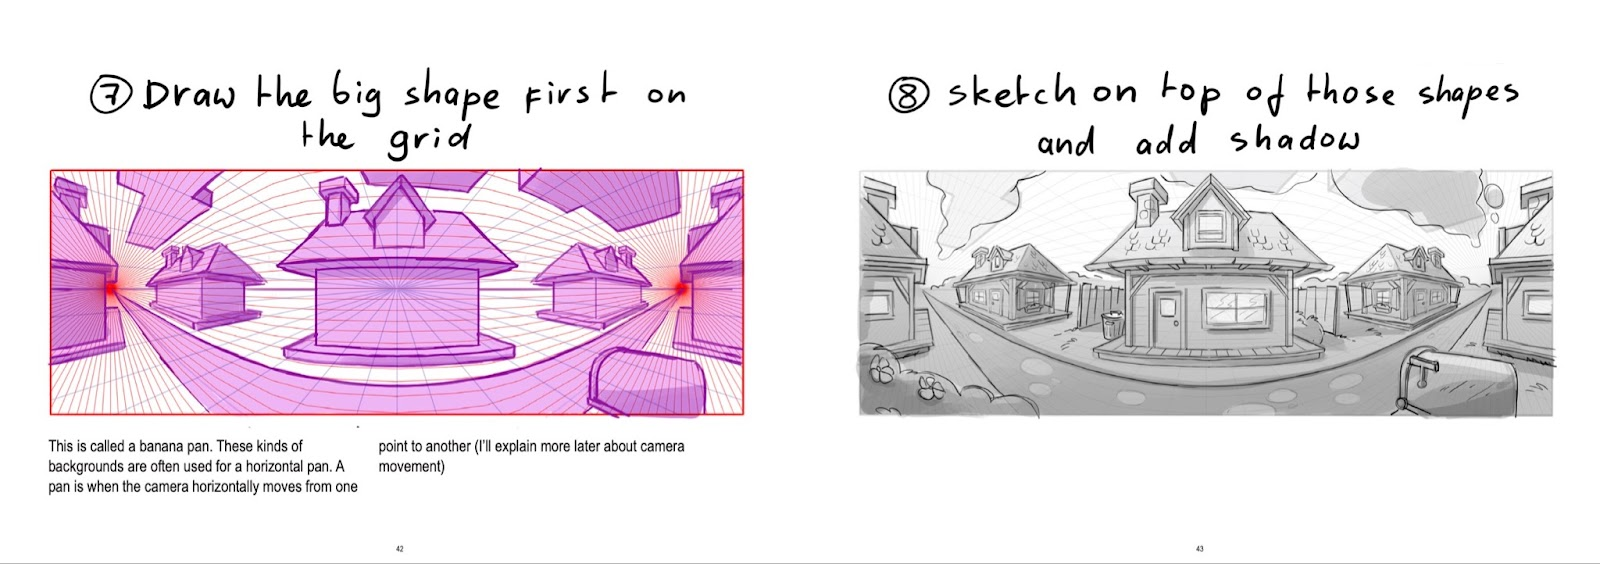
\includegraphics[width=\textwidth]{images/multi-point.jpg}}
				\caption{Виды перспективных проекций: другие (мультиточечная)}
			\end{figure}

			% Взято из  \href{
			% 	https://smirnov.school/blog/gameart/chto-takoe-linejnaya-perspektiva/
			% }{ссылка}
		}
	\end{frame}
\end{document}
\section{Преобразования наблюдения}
	\begin{frame}{Геометрические преобразования}
				
	\end{frame}